% AY2016 力学 第2問 転記（問題のみ）
\section*{第2問〔II〕}

静止している座標系 $XY$ に対して，一定の角速度 $\omega$ で回転する座標系 $X'Y'$ を
考える。座標系 $XY$ から見た平面上の点 P の位置ベクトルを $\bm{r}$，座標 $(x,y,0)$，
座標系 $X'Y'$ から見た平面上の点 P の位置ベクトルを $\bm{r}'$，座標 $(x',y',0)$ とする。

\begin{rem}
原本では冒頭が「静止している座標系 $XY$ と座標系 $XY$ に対して……」と $XY$ が
重複して書かれているが，文意から「静止している座標系 $XY$ に対して」と解した。
\end{rem}

\begin{enumerate}[label=(\arabic*)]
  \item 座標 $x$，$y$ は $x'$，$y'$，$\omega$，$t$ を用いて表せ。
  \item 座標系 $X'Y'$ から見た $X'$ 方向，$Y'$ 方向の速度成分を
        $\dot{x}'$，$\dot{y}'$，$\omega$ を用いて表せ。
  \item 点 P にある質量 $m$ の質点が外力 $\bm{F}'$ を受けて運動しているとき，
        回転座標系 $X'Y'$ から見た質点の運動方程式を求めよ。
\end{enumerate}

\begin{center}
% 図：静止系XYと角速度ωで回転する系X'Y'（角ωt）、点Pと位置ベクトル r
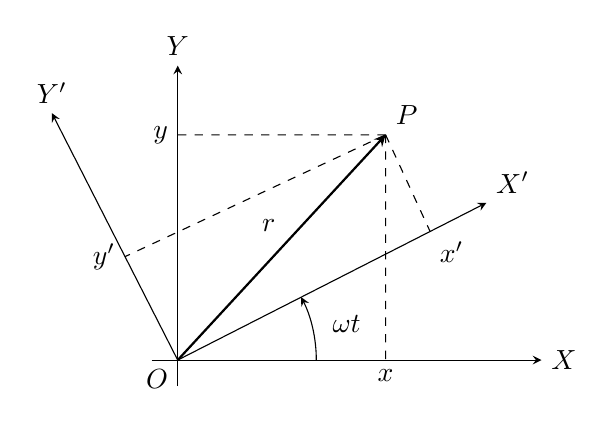
\begin{tikzpicture}[>=stealth, scale=1.1]
  \def\wt{27}
  % 静止系 XY
  \draw[->] (-0.3,0) -- (4.2,0) node[right] {$X$};
  \draw[->] (0,-0.3) -- (0,3.4) node[above] {$Y$};
  % 回転系 X'Y'（ωt 回転）
  \draw[->] (0,0) -- (\wt:4.0) node[above right] {$X'$};
  \draw[->] (0,0) -- (\wt+90:3.2) node[above] {$Y'$};
  % 点 P と位置ベクトル
  \coordinate (P) at (2.4,2.6);
  \draw[->,thick] (0,0) -- (P) node[above right] {$P$};
  \node at (1.05,1.55) {$\bm{r}$};
  % XY 成分（破線）
  \draw[dashed] (P) -- (2.4,0); \node[below] at (2.4,0) {$x$};
  \draw[dashed] (P) -- (0,2.6); \node[left] at (0,2.6) {$y$};
  % X'Y' 成分（破線：X',Y'軸への垂線の足）
  \coordinate (fx) at (\wt:3.27);   % X'軸上の足
  \coordinate (fy) at (\wt+90:1.34);% Y'軸上の足
  \draw[dashed] (P) -- (fx); \node[below right] at (fx) {$x'$};
  \draw[dashed] (P) -- (fy); \node[left] at (fy) {$y'$};
  % ωt 角
  \draw[->] (1.6,0) arc (0:\wt:1.6); \node at (1.95,0.42) {$\omega t$};
  \node[below left] at (0,0) {$O$};
\end{tikzpicture}
\end{center}
